\documentclass[11pt]{beamer}
\mode<presentation>{
\usetheme{Madrid}
\setbeamercovered{transparent}
}

\usepackage[slovak]{babel}
\usepackage[utf8]{inputenc}
\usepackage{amsmath}
\usepackage{amsthm}
\usepackage{amsfonts}
\usepackage[IL2]{fontenc}
\usepackage{graphicx}
\usepackage{lmodern}
\usepackage{hyperref}
\usepackage[ruled, czech, noline, linesnumbered, longend]{algorithm2e}
\SetAlFnt{\footnotesize}
\SetAlCapFnt{\large}
\SetAlCapNameFnt{\large}

\title{Binárny strom}
\author{Lenka Šoková}
\institute[xsokov01]{\\Vysoké učenie technické v~Brne \\Fakulta informačních technológií\\ \medskip \href{mailto:xsokov01@stud.fit.vutbr.cz}{xsokov01@stud.fit.vutbr.cz}}
\date{\scriptsize{\today}}

\begin{document}
\begin{frame}
\titlepage
\end{frame}

\begin{frame}{Motivácia}
\section{Datová štruktúra}
\textbf{Datová štruktúra} je spôsob organizácie údajov, ktorá umožnuje efektívny prístup a úpravu týchto dát.
Datové štruktúry môžme rozdeliť na \textbf{lineárne} a \textbf{nelineárne}.\\\medskip
V \textbf{lineárnej} datovej štruktúre sú údaje uložené postupne, tak že každý prvok je spojený s predchádzajúcim a nasledujúcim prvkom. Medzi lineárne datové štruktúry patrí napr. \textbf{pole}, \textbf{fronta}, \textbf{zásobní}, \textbf{viazaný zoznam}.\\\medskip
V \textbf{nelineárnej} datovej štruktúre údaje nie sú usporiadané súvisle a každý prvok môže byť prepojené aj s viac ako dvoma prvkami. Medzi nelinérne datové štruktúry patria \textbf{stromy}, \textbf{grafy}. 
\end{frame}

\begin{frame}{Základné údaje}
Strom patrí medzi \textbf{nelineárne datové štruktúry} a používa sa hierarchickú reprezentáciu dát a vzťahov medzi prvkami.\\
Binárny strom je špeciálny typ stromu v ktorom, každý uzol môže mať najviac dvoch potomkov.

\begin{figure}[ht]\label{BinaryTree}
\scalebox{0.30}{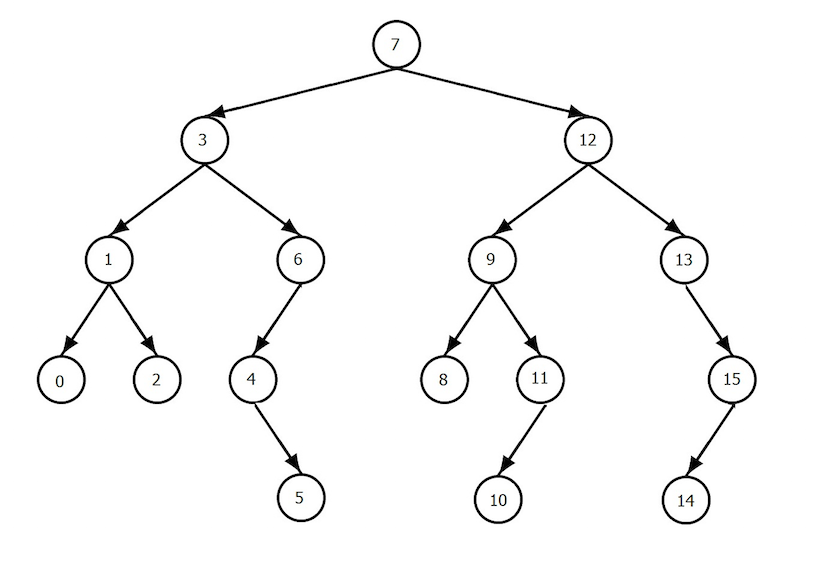
\includegraphics{binary_tree.png}}
\caption{Ilustračná štruktúra binárneho stromu}
\end{figure}
\end{frame}

\begin{frame}{Základné pojmy}
\begin{block}{Používaná terminológia}
\textbf{Root} (\emph{Koreň}) je uzol stromu, ktorý nemá žiadneho rodiča.
\\\textbf{Parent} (\emph{Rodič}) je uzol, ktorý je v hierarchii o úroveň vyššie a leží na rovnakej vetve.
\\\textbf{Child} (\emph{Dieťa}) je uzol, ktorý je priamo spojený s rodičom a v štruktúre je pod nim.
\\\textbf{Sibling} (\emph{Súrodenci}) sú uzly, ktoré majú rovnakého rodiča.
\\\textbf{Leaf} (\emph{Listy}) sú uzly, ktoré nemajú žiadne deti.
\end{block}

\end{frame}

\begin{frame}{Základné pojmy}
\begin{figure}[h] \label{BinaryTreeTerminology}
\scalebox{0.5}{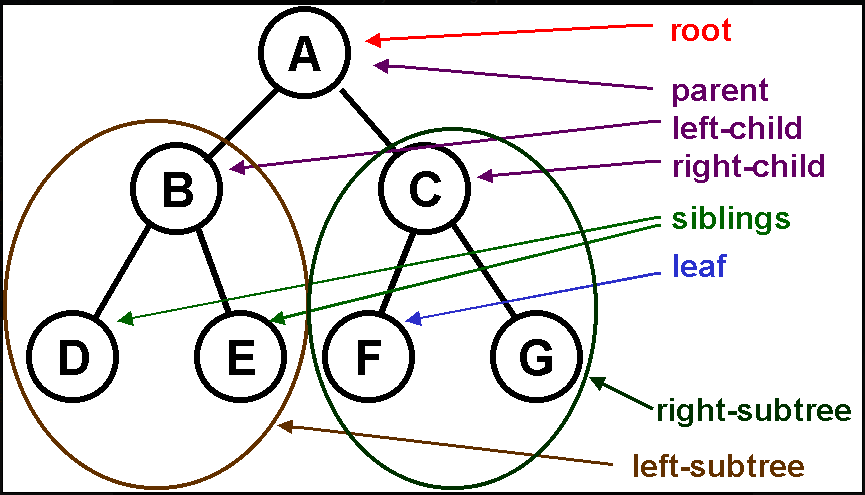
\includegraphics{binary_tree_terminology.png}}
\caption{Ilustračná štruktúra a popis terminológie binárneho stromu}
\end{figure}

\end{frame}

\begin{frame}{Základné operácie nad Binary Search Tree}
\begin{block}{Binary Search Tree - BST}
Binary Search tree (\emph{Binárny vyhľadávací strom}) je strom, v ktorom hodnota kľúča ľavého potomka je menšia ako hodnota kľúča jeho nadradeného (koreňového) uzla a hodnota kľúča pravého potomka je väčšia alebo rovná hodnote kľúča jeho nadradeného (koreňového) uzla.
\end{block}

\begin{figure}[h]\label{BST}
\scalebox{0.5}{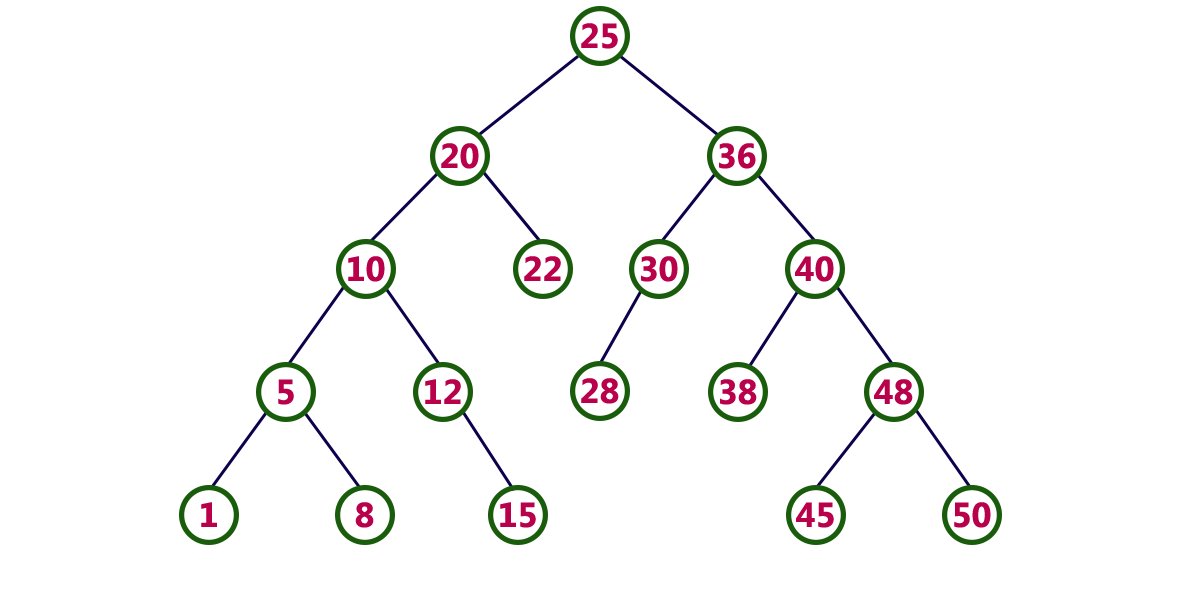
\includegraphics{BST.png}}
\caption{Ilustračná štruktúra BST}
\end{figure}
\end{frame}

\begin{frame}{Základné operácie nad Binary Search Tree}

\begin{algorithm}[H]
\caption{Search operation}\label{search}
\SetNlSkip{-1.2em}
\SetInd{1em}{1em}
\SetNlSty{}{}{:}
\SetAlgoNlRelativeSize{-1}

\KwIn{$Data$}
\KwOut{$current$}
\Indp\Indpp
\BlankLine
$struct node *current = root$\\
\While{$current\rightarrow data \neq data$}{
\If{$current \neq NULL$}{
    \eIf{$current \rightarrow data > data$}{
        $current = current \rightarrow leftChild$}
        {$current = current \rightarrow rightChild$}
    \If{$current = NULL$}{
    \KwRet{NULL}}}
}
\KwRet{$current$}
\end{algorithm}
\end{frame}



\begin{frame}{Základné operácie nad Binary Search Tree}

\begin{algorithm}[H]
\caption{Insert operation}\label{insert}
\SetNlSkip{-1.2em}
\SetInd{1em}{1em}
\SetNlSty{}{}{:}
\SetAlgoNlRelativeSize{-1}

\KwIn{$int Data$}
\Indp\Indpp
\BlankLine
\While{$True$}{
    $parent = current$\\
    \eIf{$data < parent \rightarrow data$}
    {$current = current \rightarrow leftChild$\\
        \If{$current == NULL$}{
            $parent \rightarrow leftChild = tempNode$\\
            \KwRet{}
        }}
        {$current = current\rightarrow rightChild$\\
        \If{$current == NULL$}{
            $parent\rightarrow rightChild = tempNode$\\
            \KwRet{}}
            
}}
\end{algorithm}
\end{frame}

\begin{frame}{Použité zdroje}
\begin{itemize}
    \item Binárny strom (\ref{BinaryTree}) \\ \vspace{0.5mm}
    {\footnotesize \url{https://www.mikeperham.com/2014/11/26/building-a-binary-tree-with-enumerable/}}
    \item Binárny strom - terminológia (\ref{BinaryTreeTerminology})\\
        {\footnotesize \url{https://amankrjha.blogspot.com/2012/01/data-structure-tree-and-binary-tree.html}}
    \item Binary Search Tree (\ref{BST})\\
    {\footnotesize \url{http://btechsmartclass.com/data_structures/binary-search-tree.html}}
\end{itemize}
\end{frame}
\end{document}